% Implementation chart of the attribution / reproducibility arm, in the
% format of the engine chart. Drawn 2026-09-25 from
% docs/figs/callgraph/attribution.md; entry scripts tests/attr_replicates.R
% (generator), tests/attr_metrics.R (consumer and gate), tests/attr_external.R
% (eICU), tests/attr_bands.R (bands) and run/patient_card.R (card), the
% scripts of record per the run manifests. Redrawn the same day after the
% arrow check was added to the checker: every solid arrow is backed by a row
% of the parse tables (a call, a script value read by a later statement, or
% two functions called inside one statement); the dashed `ex` arrows are
% files written by one script and read by another and are declared, not
% checked. Where a real call would have to cross a row it is stated in the
% consumer's inner-call line instead, with the box number of the callee.
% R/13b_attribution_floor.R is excluded (the old floor, not re-run); R/13 is
% present only through attribution_ranking(), which the gate imports.
% `python docs/figs/callgraph_check.py attribution` holds this chart to the
% parser-based call graph. Engine boxes are referred to by number (E 3.9 is
% box 3.9 of pipeline_implementation.tex; B 2.8 is box 2.8 of the boosters
% chart).
%
% Build:  pdflatex pipeline_attribution.tex   (from this directory)
\documentclass[10pt]{article}
\usepackage[paperwidth=44cm,paperheight=70cm,margin=8mm]{geometry}
\usepackage[T1]{fontenc}
\usepackage{lmodern}
\usepackage{amsmath}
\usepackage{tikz}
\usetikzlibrary{arrows.meta,fit,backgrounds,calc,positioning}
\pagestyle{empty}
\begin{document}
\centering
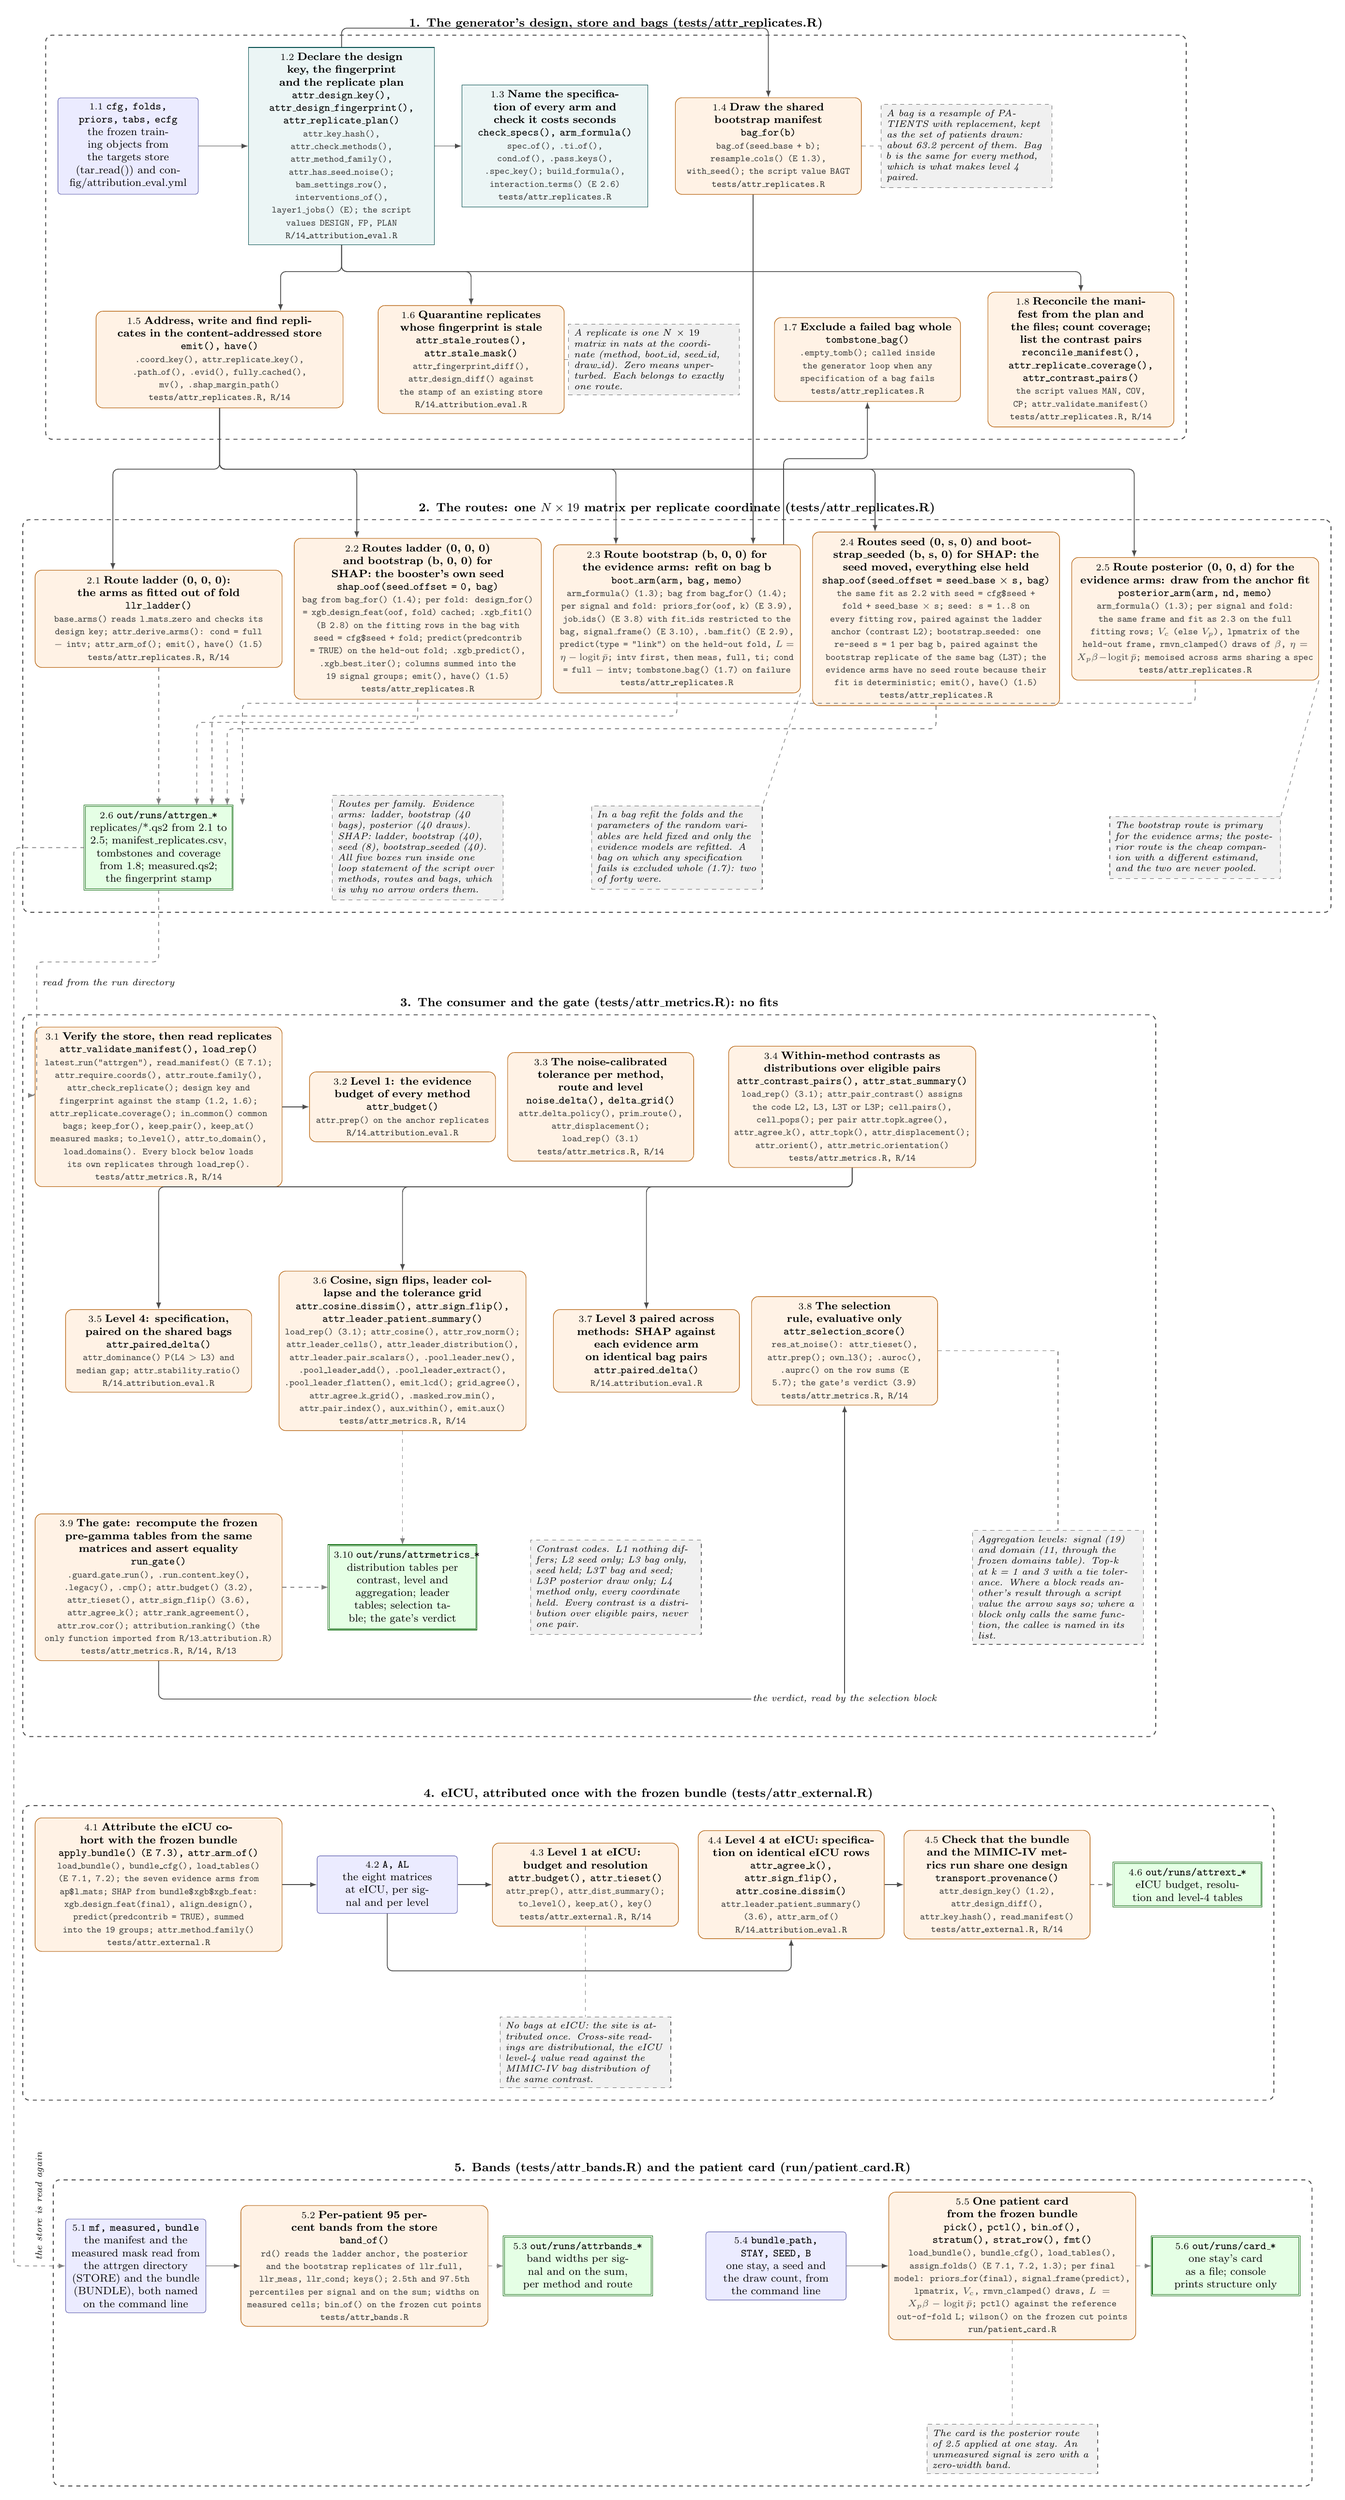
\begin{tikzpicture}[
  font=\footnotesize, x=1cm, y=1cm,
  fn/.style={draw=orange!70!black, fill=orange!10, rounded corners=5pt, align=center, inner sep=4pt, text width=4.6cm},
  fnw/.style={fn, text width=6.2cm},
  obj/.style={draw=blue!50!black!60, fill=blue!8, rounded corners=2pt, align=center, inner sep=4pt, text width=3.4cm},
  chk/.style={draw=red!60!black, fill=red!5, dashed, rounded corners=4pt, align=center, inner sep=3pt, text width=4.2cm},
  dcl/.style={draw=teal!60!black, fill=teal!8, align=center, inner sep=4pt, text width=4.6cm},
  outp/.style={draw=green!40!black, fill=green!10, double, align=center, inner sep=4pt, text width=3.6cm},
  note/.style={draw=black!60, dashed, fill=black!6, align=left, inner sep=4pt, text width=4.2cm, font=\scriptsize\itshape},
  e/.style={-{Latex[length=5pt]}, line width=0.6pt, draw=black!70, rounded corners=4pt},
  ex/.style={e, dashed, draw=black!50},
  en/.style={draw=black!55, dashed, line width=0.4pt},
  grp/.style={draw=black!70, dashed, line width=0.7pt, inner sep=9pt, rounded corners=5pt},
  lab/.style={font=\small\bfseries, anchor=south},
  al/.style={font=\scriptsize\itshape, fill=white, inner sep=1pt}]

\newcommand{\B}[5]{{\scriptsize #1}\;\textbf{#2}\\\texttt{\textbf{#3}}\\{\scriptsize\ttfamily\color{black!75}#4}\\{\scriptsize\ttfamily\color{black!80}#5}}
\newcommand{\Bs}[4]{{\scriptsize #1}\;\textbf{#2}\\\texttt{\textbf{#3}}\\{\scriptsize\ttfamily\color{black!80}#4}}
\newcommand{\Obj}[3]{{\scriptsize #1}\;\texttt{\textbf{#2}}\\#3}

% =====================================================================
% STAGE 1: the generator's design, store and bags (tests/attr_replicates.R)
% =====================================================================
\node[obj] (inp) at (2.6,0) {\Obj{1.1}{cfg, folds, priors, tabs, ecfg}{the frozen training objects from the targets store (tar\_read()) and config/attribution\_eval.yml}};
\node[dcl] (dkey) at (8.2,0) {\B{1.2}{Declare the design key, the fingerprint and the replicate plan}{attr\_design\_key(), attr\_design\_fingerprint(), attr\_replicate\_plan()}{attr\_key\_hash(), attr\_check\_methods(), attr\_method\_family(), attr\_has\_seed\_noise(); bam\_settings\_row(), interventions\_of(), layer1\_jobs() (E); the script values DESIGN, FP, PLAN}{R/14\_attribution\_eval.R}};
\node[dcl] (spec) at (13.8,0) {\B{1.3}{Name the specification of every arm and check it costs seconds}{check\_specs(), arm\_formula()}{spec\_of(), .ti\_of(), cond\_of(), .pass\_keys(), .spec\_key(); build\_formula(), interaction\_terms() (E 2.6)}{tests/attr\_replicates.R}};
\node[fn]  (bags) at (19.4,0) {\B{1.4}{Draw the shared bootstrap manifest}{bag\_for(b)}{bag\_of(seed\_base + b); resample\_cols() (E 1.3), with\_seed(); the script value BAGT}{tests/attr\_replicates.R}};
\node[note] (n1) at (24.6,0) {A bag is a resample of PATIENTS with replacement, kept as the set of patients drawn: about 63.2 percent of them. Bag $b$ is the same for every method, which is what makes level 4 paired.};

\node[fnw] (store) at (5.0,-5.6) {\B{1.5}{Address, write and find replicates in the content-addressed store}{emit(), have()}{.coord\_key(), attr\_replicate\_key(), .path\_of(), .evid(), fully\_cached(), mv(), .shap\_margin\_path()}{tests/attr\_replicates.R, R/14}};
\node[fn]  (stale) at (11.6,-5.6) {\B{1.6}{Quarantine replicates whose fingerprint is stale}{attr\_stale\_routes(), attr\_stale\_mask()}{attr\_fingerprint\_diff(), attr\_design\_diff() against the stamp of an existing store}{R/14\_attribution\_eval.R}};
\node[note] (n2) at (16.4,-5.6) {A replicate is one $N \times 19$ matrix in nats at the coordinate (method, boot\_id, seed\_id, draw\_id). Zero means unperturbed. Each belongs to exactly one route.};
\node[fn]  (tomb) at (22.0,-5.6) {\B{1.7}{Exclude a failed bag whole}{tombstone\_bag()}{.empty\_tomb(); called inside the generator loop when any specification of a bag fails}{tests/attr\_replicates.R}};
\node[fn]  (man) at (27.6,-5.6) {\B{1.8}{Reconcile the manifest from the plan and the files; count coverage; list the contrast pairs}{reconcile\_manifest(), attr\_replicate\_coverage(), attr\_contrast\_pairs()}{the script values MAN, COV, CP; attr\_validate\_manifest()}{tests/attr\_replicates.R, R/14}};

\draw[e] (inp) -- (dkey); \draw[e] (dkey) -- (spec); \draw[e] (dkey.north) -- ++(0,0.5) -| (bags.north);
\draw[en] (bags.east) -- (n1.west);
\draw[e] (dkey.south) -- ++(0,-0.7) -| ($(store.north)+(1.6,0)$);
\draw[e] (dkey.south) -- ++(0,-0.7) -| (stale.north);
\draw[e] (dkey.south) -- ++(0,-0.7) -| (man.north);
\draw[en] (stale.east) -- (n2.west);

\begin{scope}[on background layer]
\node[grp, fit=(inp)(dkey)(spec)(bags)(n1)(store)(stale)(n2)(tomb)(man), label={[lab]north:{1. The generator's design, store and bags (tests/attr\_replicates.R)}}] (b1) {};
\end{scope}

% =====================================================================
% STAGE 2: the routes, one generator loop over methods, routes and bags
% =====================================================================
\node[fnw] (ladder) at (3.4,-12.4) {\B{2.1}{Route ladder (0, 0, 0): the arms as fitted out of fold}{llr\_ladder()}{base\_arms() reads l\_mats\_zero and checks its design key; attr\_derive\_arms(): cond = full $-$ intv; attr\_arm\_of(); emit(), have() (1.5)}{tests/attr\_replicates.R, R/14}};
\node[fnw] (shap) at (10.2,-12.4) {\B{2.2}{Routes ladder (0, 0, 0) and bootstrap (b, 0, 0) for SHAP: the booster's own seed}{shap\_oof(seed\_offset = 0, bag)}{bag from bag\_for() (1.4); per fold: design\_for() = xgb\_design\_feat(oof, fold) cached; .xgb\_fit1() (B 2.8) on the fitting rows in the bag with seed = cfg\$seed + fold; predict(predcontrib = TRUE) on the held-out fold; .xgb\_predict(), .xgb\_best\_iter(); columns summed into the 19 signal groups; emit(), have() (1.5)}{tests/attr\_replicates.R}};
\node[fnw] (shapseed) at (23.8,-12.4) {\B{2.4}{Routes seed (0, s, 0) and bootstrap\_seeded (b, s, 0) for SHAP: the seed moved, everything else held}{shap\_oof(seed\_offset = seed\_base $\times$ s, bag)}{the same fit as 2.2 with seed = cfg\$seed + fold + seed\_base $\times$ s; seed: s = 1..8 on every fitting row, paired against the ladder anchor (contrast L2); bootstrap\_seeded: one re-seed s = 1 per bag b, paired against the bootstrap replicate of the same bag (L3T); the evidence arms have no seed route because their fit is deterministic; emit(), have() (1.5)}{tests/attr\_replicates.R}};
\node[fnw] (boot) at (17.0,-12.4) {\B{2.3}{Route bootstrap (b, 0, 0) for the evidence arms: refit on bag b}{boot\_arm(arm, bag, memo)}{arm\_formula() (1.3); bag from bag\_for() (1.4); per signal and fold: priors\_for(oof, k) (E 3.9), job\_ids() (E 3.8) with fit\_ids restricted to the bag, signal\_frame() (E 3.10), .bam\_fit() (E 2.9), predict(type = "link") on the held-out fold, $L = \eta - \operatorname{logit}\bar p$; intv first, then meas, full, ti; cond = full $-$ intv; tombstone\_bag() (1.7) on failure}{tests/attr\_replicates.R}};
\node[fnw] (post) at (30.6,-12.4) {\B{2.5}{Route posterior (0, 0, d) for the evidence arms: draw from the anchor fit}{posterior\_arm(arm, nd, memo)}{arm\_formula() (1.3); per signal and fold: the same frame and fit as 2.3 on the full fitting rows; $V_c$ (else $V_p$), lpmatrix of the held-out frame, rmvn\_clamped() draws of $\beta$, $\eta = X_p\beta - \operatorname{logit}\bar p$; memoised across arms sharing a spec}{tests/attr\_replicates.R}};

\node[outp] (gen) at (3.4,-18.4) {\Obj{2.6}{out/runs/attrgen\_*}{replicates/*.qs2 from 2.1 to 2.5; manifest\_replicates.csv, tombstones and coverage from 1.8; measured.qs2; the fingerprint stamp}};
\node[note] (n3) at (10.2,-18.4) {Routes per family. Evidence arms: ladder, bootstrap (40 bags), posterior (40 draws). SHAP: ladder, bootstrap (40), seed (8), bootstrap\_seeded (40). All five boxes run inside one loop statement of the script over methods, routes and bags, which is why no arrow orders them.};
\node[note] (n4) at (17.0,-18.4) {In a bag refit the folds and the parameters of the random variables are held fixed and only the evidence models are refitted. A bag on which any specification fails is excluded whole (1.7): two of forty were.};
\node[note] (n5) at (30.6,-18.4) {The bootstrap route is primary for the evidence arms; the posterior route is the cheap companion with a different estimand, and the two are never pooled.};

% the store serves every route (1.5 -> 2.x): a bus below stage 1
\draw[e] (store.south) -- ++(0,-1.6) -| ($(ladder.north)+(-1.2,0)$);
\draw[e] (store.south) -- ++(0,-1.6) -| ($(shap.north)+(-1.6,0)$);
\draw[e] (store.south) -- ++(0,-1.6) -| ($(boot.north)+(-1.6,0)$);
\draw[e] (store.south) -- ++(0,-1.6) -| ($(shapseed.north)+(-1.6,0)$);
\draw[e] (store.south) -- ++(0,-1.6) -| ($(post.north)+(-1.6,0)$);
% the bags reach the bootstrap routes (1.4 -> 2.3), the failed bag is tombstoned (2.3 -> 1.7)
\draw[e] ($(bags.south)+(-0.4,0)$) -- ($(boot.north)+(2.0,0)$);
\draw[e] ($(boot.north)+(2.8,0)$) |- (22.0,-8.2) -- (tomb.south);
% written to the run directory
\draw[ex] (ladder.south) -- (gen.north);
\draw[ex] (shap.south) -- ++(0,-0.6) -| ($(gen.north)+(1.0,0)$);
\draw[ex] (boot.south) -- ++(0,-0.6) -| ($(gen.north)+(1.4,0)$);
\draw[ex] (shapseed.south) -- ++(0,-0.6) -| ($(gen.north)+(1.8,0)$);
\draw[ex] (post.south) -- ++(0,-0.6) -| ($(gen.north)+(2.2,0)$);
\draw[en] (boot.south east) -- (n4.north east);
\draw[en] (post.south east) -- (n5.north east);

\begin{scope}[on background layer]
\node[grp, fit=(ladder)(shap)(boot)(shapseed)(post)(n3)(gen)(n4)(n5), label={[lab]north:{2. The routes: one $N \times 19$ matrix per replicate coordinate (tests/attr\_replicates.R)}}] (b2) {};
\end{scope}

% =====================================================================
% STAGE 3: the consumer (tests/attr_metrics.R): fits nothing
% =====================================================================
\node[fnw] (verify) at (3.4,-25.2) {\B{3.1}{Verify the store, then read replicates}{attr\_validate\_manifest(), load\_rep()}{latest\_run("attrgen"), read\_manifest() (E 7.1); attr\_require\_coords(), attr\_route\_family(), attr\_check\_replicate(); design key and fingerprint against the stamp (1.2, 1.6); attr\_replicate\_coverage(); in\_common() common bags; keep\_for(), keep\_pair(), keep\_at() measured masks; to\_level(), attr\_to\_domain(), load\_domains(). Every block below loads its own replicates through load\_rep().}{tests/attr\_metrics.R, R/14}};
\node[fn]  (l1) at (9.8,-25.2) {\B{3.2}{Level 1: the evidence budget of every method}{attr\_budget()}{attr\_prep() on the anchor replicates}{R/14\_attribution\_eval.R}};
\node[fn]  (noise) at (15.0,-25.2) {\B{3.3}{The noise-calibrated tolerance per method, route and level}{noise\_delta(), delta\_grid()}{attr\_delta\_policy(), prim\_route(), attr\_displacement(); load\_rep() (3.1)}{tests/attr\_metrics.R, R/14}};
\node[fnw] (within) at (21.6,-25.2) {\B{3.4}{Within-method contrasts as distributions over eligible pairs}{attr\_contrast\_pairs(), attr\_stat\_summary()}{load\_rep() (3.1); attr\_pair\_contrast() assigns the code L2, L3, L3T or L3P; cell\_pairs(), cell\_pops(); per pair attr\_topk\_agree(), attr\_agree\_k(), attr\_topk(), attr\_displacement(); attr\_orient(), attr\_metric\_orientation()}{tests/attr\_metrics.R, R/14}};

\node[fn]  (l4) at (3.4,-31.6) {\B{3.5}{Level 4: specification, paired on the shared bags}{attr\_paired\_delta()}{attr\_dominance() P(L4 $>$ L3) and median gap; attr\_stability\_ratio()}{R/14\_attribution\_eval.R}};
\node[fnw] (lead) at (9.8,-31.6) {\B{3.6}{Cosine, sign flips, leader collapse and the tolerance grid}{attr\_cosine\_dissim(), attr\_sign\_flip(), attr\_leader\_patient\_summary()}{load\_rep() (3.1); attr\_cosine(), attr\_row\_norm(); attr\_leader\_cells(), attr\_leader\_distribution(), attr\_leader\_pair\_scalars(), .pool\_leader\_new(), .pool\_leader\_add(), .pool\_leader\_extract(), .pool\_leader\_flatten(), emit\_lcd(); grid\_agree(), attr\_agree\_k\_grid(), .masked\_row\_min(), attr\_pair\_index(), aux\_within(), emit\_aux()}{tests/attr\_metrics.R, R/14}};
\node[fn]  (cross) at (16.2,-31.6) {\Bs{3.7}{Level 3 paired across methods: SHAP against each evidence arm on identical bag pairs}{attr\_paired\_delta()}{R/14\_attribution\_eval.R}};
\node[fn]  (sel) at (21.4,-31.6) {\B{3.8}{The selection rule, evaluative only}{attr\_selection\_score()}{res\_at\_noise(): attr\_tieset(), attr\_prep(); own\_l3(); .auroc(), .auprc() on the row sums (E 5.7); the gate's verdict (3.9)}{tests/attr\_metrics.R, R/14}};

\node[fnw] (gate) at (3.4,-37.8) {\B{3.9}{The gate: recompute the frozen pre-gamma tables from the same matrices and assert equality}{run\_gate()}{.guard\_gate\_run(), .run\_content\_key(), .legacy(), .cmp(); attr\_budget() (3.2), attr\_tieset(), attr\_sign\_flip() (3.6), attr\_agree\_k(); attr\_rank\_agreement(), attr\_row\_cor(); attribution\_ranking() (the only function imported from R/13\_attribution.R)}{tests/attr\_metrics.R, R/14, R/13}};
\node[outp] (met) at (9.8,-37.8) {\Obj{3.10}{out/runs/attrmetrics\_*}{distribution tables per contrast, level and aggregation; leader tables; selection table; the gate's verdict}};
\node[note] (n6) at (15.4,-37.8) {Contrast codes. L1 nothing differs; L2 seed only; L3 bag only, seed held; L3T bag and seed; L3P posterior draw only; L4 method only, every coordinate held. Every contrast is a distribution over eligible pairs, never one pair.};
\node[note] (n7) at (27.0,-37.8) {Aggregation levels: signal (19) and domain (11, through the frozen domains table). Top-k at k = 1 and 3 with a tie tolerance. Where a block reads another's result through a script value the arrow says so; where a block only calls the same function, the callee is named in its list.};

\draw[e] (verify) -- (l1);
\draw[e] (within.south) -- ++(0,-0.5) -| (cross.north);
\draw[e] (within.south) -- ++(0,-0.5) -| (lead.north);
\draw[e] (within.south) -- ++(0,-0.5) -| (l4.north);
\draw[e] (gate.south) -- ++(0,-1.0) -| (sel.south) node[al, pos=0.5] {the verdict, read by the selection block};
\draw[ex] (lead) -- (met); \draw[ex] (gate) -- (met);
\draw[en] (sel.east) -| (n7.north);
\draw[ex] (gen.south) |- (0.2,-21.4) |- ($(verify.west)+(0,0.3)$) node[al, pos=0.08, anchor=west] {~read from the run directory};

\begin{scope}[on background layer]
\node[grp, fit={(verify)(l1)(noise)(within)(l4)(lead)(cross)(sel)(gate)(met)(n6)(n7)(12.0,-41.4)}, label={[lab]north:{3. The consumer and the gate (tests/attr\_metrics.R): no fits}}] (b3) {};
\end{scope}

% =====================================================================
% STAGE 4: eICU (tests/attr_external.R)
% =====================================================================
\node[fnw] (ext) at (3.4,-45.6) {\B{4.1}{Attribute the eICU cohort with the frozen bundle}{apply\_bundle() (E 7.3), attr\_arm\_of()}{load\_bundle(), bundle\_cfg(), load\_tables() (E 7.1, 7.2); the seven evidence arms from ap\$l\_mats; SHAP from bundle\$xgb\$xgb\_feat: xgb\_design\_feat(final), align\_design(), predict(predcontrib = TRUE), summed into the 19 groups; attr\_method\_family()}{tests/attr\_external.R}};
\node[obj] (A) at (9.4,-45.6) {\Obj{4.2}{A, AL}{the eight matrices at eICU, per signal and per level}};
\node[fn]  (extl1) at (14.6,-45.6) {\B{4.3}{Level 1 at eICU: budget and resolution}{attr\_budget(), attr\_tieset()}{attr\_prep(), attr\_dist\_summary(); to\_level(), keep\_at(), key()}{tests/attr\_external.R, R/14}};
\node[fn]  (extl4) at (20.0,-45.6) {\B{4.4}{Level 4 at eICU: specification on identical eICU rows}{attr\_agree\_k(), attr\_sign\_flip(), attr\_cosine\_dissim()}{attr\_leader\_patient\_summary() (3.6), attr\_arm\_of()}{R/14\_attribution\_eval.R}};
\node[fn]  (prov) at (25.4,-45.6) {\B{4.5}{Check that the bundle and the MIMIC-IV metrics run share one design}{transport\_provenance()}{attr\_design\_key() (1.2), attr\_design\_diff(), attr\_key\_hash(), read\_manifest()}{tests/attr\_external.R, R/14}};
\node[outp] (extout) at (30.4,-45.6) {\Obj{4.6}{out/runs/attrext\_*}{eICU budget, resolution and level-4 tables}};
\node[note] (n8) at (14.6,-50.0) {No bags at eICU: the site is attributed once. Cross-site readings are distributional, the eICU level-4 value read against the MIMIC-IV bag distribution of the same contrast.};

\draw[e] (ext) -- (A); \draw[e] (A) -- (extl1);
\draw[e] (A.south) -- ++(0,-1.5) -| (extl4.south);
\draw[e] (extl4) -- (prov); \draw[ex] (prov) -- (extout);
\draw[en] (extl1.south) -- (n8.north);

\begin{scope}[on background layer]
\node[grp, fit=(ext)(A)(extl1)(extl4)(prov)(extout)(n8), label={[lab]north:{4. eICU, attributed once with the frozen bundle (tests/attr\_external.R)}}] (b4) {};
\end{scope}

% =====================================================================
% STAGE 5: bands and the patient card
% =====================================================================
\node[obj] (bandsin) at (2.8,-55.6) {\Obj{5.1}{mf, measured, bundle}{the manifest and the measured mask read from the attrgen directory (STORE) and the bundle (BUNDLE), both named on the command line}};
\node[fnw] (bands) at (8.8,-55.6) {\B{5.2}{Per-patient 95 percent bands from the store}{band\_of()}{rd() reads the ladder anchor, the posterior and the bootstrap replicates of llr\_full, llr\_meas, llr\_cond; keys(); 2.5th and 97.5th percentiles per signal and on the sum; widths on measured cells; bin\_of() on the frozen cut points}{tests/attr\_bands.R}};
\node[outp] (bandsout) at (14.4,-55.6) {\Obj{5.3}{out/runs/attrbands\_*}{band widths per signal and on the sum, per method and route}};
\node[obj] (cardin) at (19.6,-55.6) {\Obj{5.4}{bundle\_path, STAY, SEED, B}{one stay, a seed and the draw count, from the command line}};
\node[fnw] (card) at (25.8,-55.6) {\B{5.5}{One patient card from the frozen bundle}{pick(), pctl(), bin\_of(), stratum(), strat\_row(), fmt()}{load\_bundle(), bundle\_cfg(), load\_tables(), assign\_folds() (E 7.1, 7.2, 1.3); per final model: priors\_for(final), signal\_frame(predict), lpmatrix, $V_c$, rmvn\_clamped() draws, $L = X_p\beta - \operatorname{logit}\bar p$; pctl() against the reference out-of-fold L; wilson() on the frozen cut points}{run/patient\_card.R}};
\node[outp] (cardout) at (31.4,-55.6) {\Obj{5.6}{out/runs/card\_*}{one stay's card as a file; console prints structure only}};
\node[note] (n9) at (25.8,-60.4) {The card is the posterior route of 2.5 applied at one stay. An unmeasured signal is zero with a zero-width band.};

\draw[e] (bandsin) -- (bands); \draw[ex] (bands) -- (bandsout);
\draw[e] (cardin) -- (card); \draw[ex] (card) -- (cardout);
\draw[en] (card.south) -- (n9.north);
\draw[ex] (gen.west) -- (-0.4,-18.4) -- (-0.4,-55.6) -- (bandsin.west) node[al, pos=0.5, anchor=west, rotate=90] {~the store is read again};

\begin{scope}[on background layer]
\node[grp, fit=(bandsin)(bands)(bandsout)(cardin)(card)(cardout)(n9), label={[lab]north:{5. Bands (tests/attr\_bands.R) and the patient card (run/patient\_card.R)}}] (b5) {};
\end{scope}
\end{tikzpicture}
\end{document}
